\clearpage
\section{Material and methods}
\label{sec:simulations-methodology}
%%%%%

In this section we describe the respective benchmarks and related methodology in detail.

%%
\subsection{Simulations}
\label{subsec:simulations-methods}
%%

We consider a range of simulation studies with various deterministic synthetic covariance structures.
We take full advantage of the flexibility that simulations offer, and explore a wide range of data (e.g.~dimensionalities and noise configurations) and estimation method (e.g.~hyperparameters and post-hoc analysis) characteristics.
The synthetic covariance structures are both designed for exploring edge cases as well as mimicking structures that we may expect to drive actual processes in the human brain.

%%
\subsubsection{Synthetic covariance structures}
\label{subsec:synthetic-covariance-structures}
%%

Perhaps surprisingly, the covariance structures to be expected in real data are rarely discussed.
The coupling of \gls{bold} time series is, in fact, still a black box to a large degree.
In lieu of known covariance structure we test models against a battery of possible and reasonably exhaustive (synthetic) structures that may be encountered in an \gls{fmri} scan.
The covariance structures studied are shown in \cref{fig:synthetic-covariance-structures};
null covariance (node time series are uncorrelated during the entire scan),
a constant (i.e.~static) covariance of $\sigma_{ij} = 0.8$,
periodic covariance structures (a slowly oscillating sine wave defined by one period, and a fast one with three periods) that model transient changes in coupling,
a stepwise covariance that models two sudden (large) change points in covariance,
a covariance structure that simulates a series of state transitions, as inspired by~\textcite{Thompson2018},
and finally a covariance structure inspired by the \gls{tb-fmri} visual checkerboard task we study (see \cref{subsec:rockland-methodology}).
This last covariance structure mimics the presence and absence of an external visual stimulus (assuming it would show up as such in the covariance structure).
It is designed by taking the convolution between the \gls{hrf} and the respective stimulus block design.


\begin{figure}[t]
  \centering
  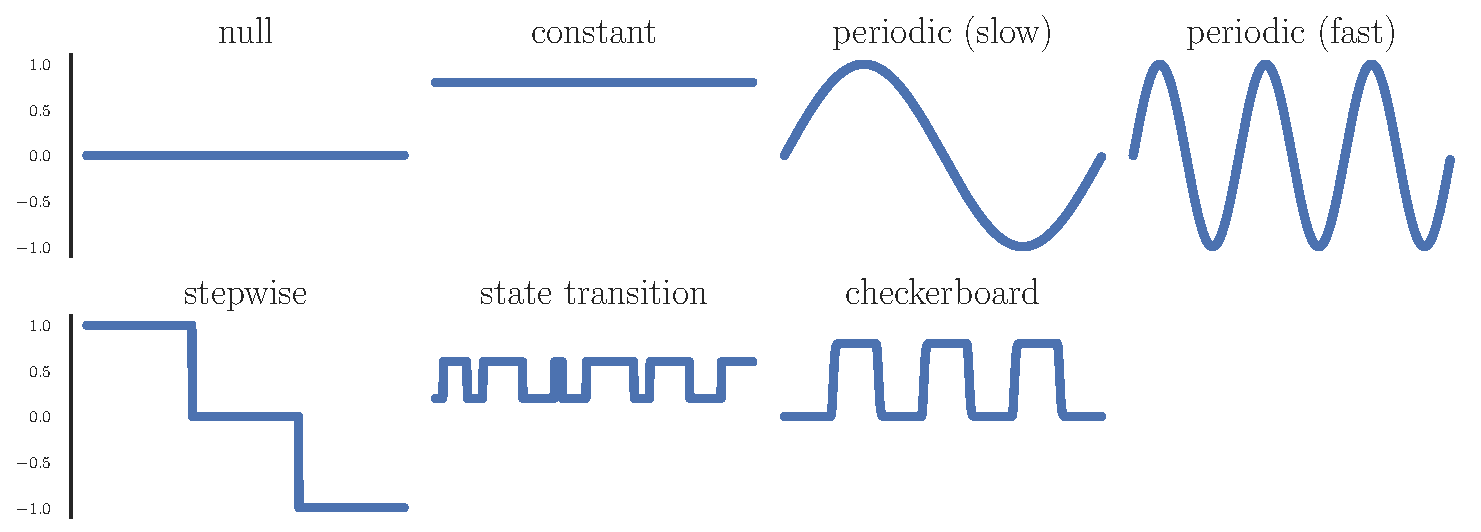
\includegraphics[width=\textwidth]{fig/sim/covariance_structures}
  \caption{
    Synthetic covariance structures considered in the simulations benchmark, capturing a wide range of edge cases and potentially realistic covariance structures.
  }
  \label{fig:synthetic-covariance-structures}
\end{figure}


%%
\subsubsection{Data generation}
%%

Data is simulated as follows.
We sample observations $\mathbf{y}_n \in \mathbb{R}^D$ at each time step~$1 \leq n \leq N$ from a zero-mean Gaussian distribution:
\begin{equation}
  \mathbf{y}_n \sim \mathcal{N}(\mathbf{0}, \mathbf{\Sigma}_n),
  \label{eq:data-generation}
\end{equation}
for a given covariance matrix $\mathbf{\Sigma}_n$ at time step $n$.
This covariance matrix depends on the synthetic covariance structure parameters defining the data set.
All time series are subsequently individually normalized to have mean zero and unit standard deviation.

The number of time series ($D$) we expect to see in practice depends on the experimental design and research question at hand.
In most applications more than two nodes or components are studied.
Some studies even consider voxel time series directly, in which case $D$ can be in the hundreds of thousands or even millions.
Here, we test on pairwise (i.e.~\emph{bivariate}; $D = 2$) data, as well as on a trivariate ($D = 3$) data sets.
Ideally we want to study \gls{tvfc} estimation performance per method \emph{as a function of} dimensionality.
The trivariate case serves as an intermediate step toward scaling up to higher dimensions.
All simulation experiments are run $T = 200$ times, and model performance is averaged across these trials.

The bivariate benchmark analyses are similar to the ones conducted by~\textcite{Lindquist2014}.
Furthermore, they will serve as a blueprint for when we analyze connectivity between just two brain regions.
It is important to note that methods based on \gls{sw} are always pairwise as well.
Thus, if a method robustly and consistently outperforms \gls{sw} on bivariate data, it will do so on higher dimensional data as well if we were to simply loop over all pairs of time series.

Our covariance structure for generating bivariate data (\cref{eq:data-generation}) is given by
\begin{equation}
  \mathbf{\Sigma}_n = \begin{bmatrix}
    1 & \sigma(n) \\
    \sigma(n) & 1
  \end{bmatrix},
\end{equation}
where the covariance term $\sigma(n)$ varies across time according to the various covariance structures shown in \cref{fig:synthetic-covariance-structures}.
For the bivariate case, $\sigma(n)$ is allowed to fall within range~[-1,1], to maintain a positive semi-definite matrix.
As mentioned before, since the diagonal consists of ones, these covariance matrices are identical to their respective correlation matrices.

For the trivariate data, we implement both a fully co-varying (i.e.~\emph{dense}) covariance structure
\begin{equation}
  \mathbf{\Sigma}_n = \begin{bmatrix}
    1 & \sigma(n) & \sigma(n) \\
    \sigma(n) & 1 & \sigma(n) \\
    \sigma(n) & \sigma(n) & 1
  \end{bmatrix},
\end{equation}
and a \emph{sparse} version where only the first two time series are correlated
\begin{equation}
  \mathbf{\Sigma}_n = \begin{bmatrix}
    1 & \sigma(n) & 0 \\
    \sigma(n) & 1 & 0 \\
    0 & 0 & 1
  \end{bmatrix},
\end{equation}
where the covariance terms $\sigma(n)$ again vary across time as depicted in \cref{fig:synthetic-covariance-structures}.
This sparse version can be considered alike to the bivariate case with an added uncorrelated (i.e.~control) region.
Perhaps we would expect such structure (most edges being stationary, but some showing time-varying structure) in \gls{fmri} data, but yet again lacking a ground truth makes this unclear.
To keep the covariance matrices positive semi-definite, the allowed range for $\sigma(n)$ in the dense trivariate case is~$[-0.5,1]$ while for the sparse version it remains~$[-1,1]$.

We want our results to be robust across data set lengths.
\gls{fmri} scans (whether \gls{rs-fmri} or \gls{tb-fmri}) are typically in the order of~240 to~1,200 seconds; participants can only be kept in a scanner for a limited amount of time.
The \gls{tr} of scanning setups typically ranges from~0.5 to~2 seconds.
Combining these ranges gives us a range of the number of data points $N$ we expect to see in practice.
Therefore, we study the cases of $N \in \{120, 200, 400, 1200\}$ data points per time series.
We report results for $N = 400$, because this is the closest to the values of $N$ in \cref{ch:ukb} and thus most representative.
Results for other values of $N$ are retired to \cref{appendix:more-benchmarking-results}.
It is important to be aware of the typical trade-off where scans with higher \glspl{tr} consist of fewer data points, although these are usually observed with less noise.
We also note that Bayesian methods typically perform better on smaller data sets.
Even though we strive to find a robust method that can be used in any setting, we consider the option that some methods may work better with smaller but less noisy data sets and other methods may perform better with larger, noisy data sets.
This style of analysis is reminiscient of the multiverse analysis~\parencite{Steegen2016}, as discussed in more detail in \cref{subsec:robustness}.

%%
\subsubsection{Noise addition and hybrid simulations}
%%

The human nervous system is subject to various sources of noise, such as Brownian motion in synapses and ion channels~\parencite{Faisal2008}.
\gls{fmri} scanners are imperfect machines and introduce further sources of noise as well.
These account for system noise and observational noise.
Taken together this makes \gls{fmri} data (in)famously noisy~\parencite[see also][for analysis and biophysical simulations of impact of noise and delay]{Deco2009}.
The noise is both spatially and temporally correlated.

To make our benchmark more robust, all experiments are repeated on the data sets described priorly with added noise.
Noise ensures generalizability of any conclusion we make.
Higher levels of noise can also be interpreted as decreasing the amplitude of any existing covariance structure, requiring methods to be increasingly sensitive.
In an extensive literature review, \textcite{Welvaert2013} found \gls{snr} values in \gls{fmri} data to range between 0.35 and 203.6.
Higher \glspl{snr} are preferred in practice.
%
Here, all experiments are repeated with added noise with an \gls{snr} $\in \{1, 2, 6\}$.
Lower \glspl{snr} showed all \gls{tvfc} estimation methods breaking down, and higher \glspl{snr} yielded equivalent results to the noiseless case.

We study two types of added noise.
The simplest case (white noise) can be considered similar to thermal noise in \gls{fmri} scanners.
Secondly, in the \emph{hybrid} simulations, we use an \gls{rs-fmri} data set to add noise to the synthetically generated activation data.
We use data from the \gls{hcp} data set as described in more detail in \cref{subsec:data-hcp}.
If we take time series from brain regions (or \gls{ica} components) from different subjects and add them to the synthetic signal, we can assume that no additional covariance structure is added.
These \gls{rs-fmri} time series are selected from the middle of the scans.
Such hybrid simulations are similar in spirit to \textcite{Keilholz2013}, where subject scan session IDs are randomized to ensure a proper null model for a statistical test.
The benefit of this is that we preserve typical \gls{fmri} time series characteristics.
For \gls{rs-fmri} data this typically includes heavy spatial and temporal autocorrelation~\parencite{Keilholz2017}, which has been shown to affect \gls{tvfc} estimates~\parencite{Honari2019}.
This is contrasted to \textcite{Thompson2018}, where autocorrelation is specified and simulated in the data directly.
We argue that since we do not know what a realistic level of autocorrelation would be, using real data autocorrelation is preferred.

In both noise addition routines, we consider our noisy $\mathbf{y}_n^*$ to be a linear mix of noiseless signal $\mathbf{y}_n$ (as defined above) and (independent) noise time series $\mathbf{\epsilon}_n$:
\begin{equation}
  \mathbf{y}_n^* = \alpha \mathbf{y}_n + (1 - \alpha) \mathbf{\epsilon}_n,
\end{equation}
where $0 < \alpha < 1$ is called the mixing coefficient, with the \gls{snr} being equal to $\frac{\alpha}{1-\alpha}$.

Adding noise affects the signal (ground truth) variances and covariances.
The time series variances and covariances are updated as follows.

In the case of white noise, $\mathbf{\epsilon}_n \sim \mathcal{N}(\mathbf{0}, \mathbf{I})$.
To understand what will happen to the variances of each time series, we firstly note that
\begin{equation}
  \mathbb{E}[\mathbf{y}_n^*] = \alpha \mathbb{E}[\mathbf{y}_n] + (1-\alpha)\mathbb{E}[\mathbf{\epsilon}_n] = \mathbf{0}.
\end{equation}
This means that the new time series variance is
\begin{equation}
  \begin{split}
    \sigma_{y_n^*}^2 & = \mathbb{E}[(\mathbf{y}_n^*)^2] - (\mathbb{E}[\mathbf{y}_n^*])^2 = \mathbb{E}[(\mathbf{y}_n^*)^2] \\
    & = \mathbb{E}[\alpha^2 \mathbf{y}_n^2 + 2\alpha(1-\alpha)y_n\mathbf{\epsilon}_n + (1-\alpha)^2\mathbf{\epsilon}_n^2] \\
    & = \alpha^2\mathbb{E}[\mathbf{y}_n^2] + (1-\alpha)^2\mathbb{E}[\mathbf{\epsilon}_n^2] \\
    & = \alpha^2 + (1-\alpha)^2.
  \end{split}
\end{equation}
Regarding the covariance terms, all cross-terms except within $\mathbf{y}_n$ are zero, so we are simply left with $\sigma_{y_{n,1}^*y_{n,2}^*} = \alpha^2\sigma_{y_{n,1}y_{n,2}}$.
To maintain the time series variances $\sigma_{y_t^*}^2$ being equal to 1, we compute the new (noisy) signal as given by
\begin{equation}
  \mathbf{y}_n^* = \frac{1}{\sqrt{\alpha^2 + (1-\alpha)^2}} [\alpha \mathbf{y}_n + (1 - \alpha) \mathbf{\epsilon}_n],
\end{equation}
so that our new ``ground truth'' covariance terms are updated as
\begin{equation}
  \sigma_{y_{n,1}^*y_{n,2}^*} = \frac{\alpha^2}{\alpha^2 + (1-\alpha)^2} \sigma_{y_{n,1}y_{n,2}}.
\end{equation}

In the hybrid experiments, we adjust the ground truth covariances in the same way as with white noise.
Although the distribution of the noise is not known, we know that $\mathbb{E}[\epsilon] = 0$ and $\mathbb{E}[\epsilon^2] = 1$, since we normalized it as such.

%%
\subsubsection{Evaluation and performance metrics}
%%

Comparing model estimates visually provides an initial overview of method performance and qualitative characteristics.
To \emph{quantify} performance we compute the \gls{rmse} between estimated and ground truth Pearson correlation, following~\textcite{Wilson2010, Lindquist2014}.
This can be considered a \emph{reconstruction} loss.
Estimators with lower \gls{rmse} will be considered superior estimators.
For the trivariate cases, we compute the \gls{rmse} across all elements of the full correlation matrices.

%%
\subsubsection{Imputation benchmark}
%%

We run the imputation benchmark as described in \cref{subsec:imputation-benchmark}.
Of course, it is unnecessary to do so, because we have the actual underlying ground truth.
However, this allows us to investigate the relationship between method performance on this imputation benchmark and its ability to recover an actual ground truth.

%%
\subsection{Resting-state fMRI}
%%

\info[inline]{Paragraph: Introduce rs-fMRI-based benchmarks.}
Here we study how an \gls{rs-fmri} data set can be used to benchmark \gls{tvfc} estimation methods.
We look at different (common) classes of benchmarks based on \gls{rs-fmri} data: the prediction of subject measures, test-retest robustness, and the imputation benchmark as described in \cref{subsec:imputation-benchmark}.
For the latter we are especially interested in its relationship with the other benchmarks.
We use a single source of data for all these \gls{rs-fmri} benchmarks: the \gls{hcp}.
Moreover, we conduct a brain state analysis.
This analysis is more suited as demonstration rather than benchmark.

%%
\subsubsection{Data: Human Connectome Project}
\label{subsec:data-hcp}
%%

The \gls{hcp} has collected a large, publicly available data set.
It is one of the largest and most commonly used data sets in neuroimaging research~\parencite{VanEssen2012, VanEssen2013, Elam2021}.
It is important to use publicly available and transparently collected data to benchmark methods.
Participants in this data set are relatively young adults, aged 22-37.
The data collection and collaboration of this project were accompanied by fundamental technological advances underlying scan collection.
This included advances in the domains of accelerated multiband and multiplexed \gls{epi} pulse sequences~\parencite{Moeller2010, Feinberg2010, Setsompop2012, Xu2012}.

More specifically, we use data from the \gls{hcp} S1200 public release (published in March 2017).
All scans are acquired with a 3T Siemens connectome-Skyra using a multi-band sequence.
The readily available $D = 15$ dimensional \gls{ica} based node time series are used.
\Gls{ica} is a technique that decomposes observed (voxel) time series into a set of independent components.
The original individual observed time series can then be reconstructed as a mix of these components.
Each of these \gls{ica} time series thus represents a significant \emph{component} of whole-brain activity.
Other dimensionalities $D \in \{50,100,200,300\}$ are also readily available.
We opted to study $D = 15$ time series, representative of the number of time series studied in many cognitive studies.
For example, our depression study in \cref{ch:ukb} studies both nine and three time series.
%
For interpretability, each \gls{ica} component is mapped to a well-known \gls{fn}, following \textcite{Giorgio2018}.
We asked three neuroimaging researchers to visually inspect and manually assign each \gls{ica} component to one of the networks from \cref{fig:brainmap-functional-networks}; networks that resemble task-driven \glspl{fn}~\parencite{Fox2007, Smith2009}.


% Remove a), b), etc.
\captionsetup[subfigure]{labelformat=empty}

\begin{figure}[t]
  \centering
  \subcaptionbox{1: Visual (Medial) \label{fig:rsn-1}}{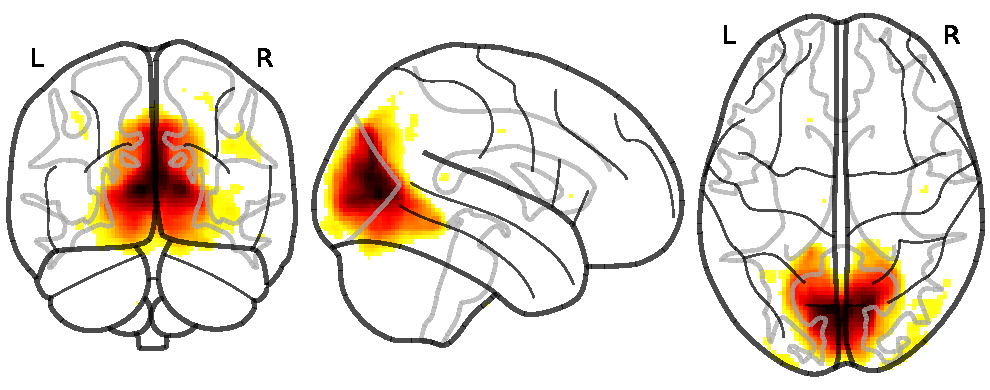
\includegraphics[width=0.38\textwidth]{fig/hcp/RSN_components/RSN_00}}
  \hspace{0.08\textwidth}
  \subcaptionbox{2: Visual (Occipital, Cognition–Language–Orthography) \label{fig:rsn-2}}{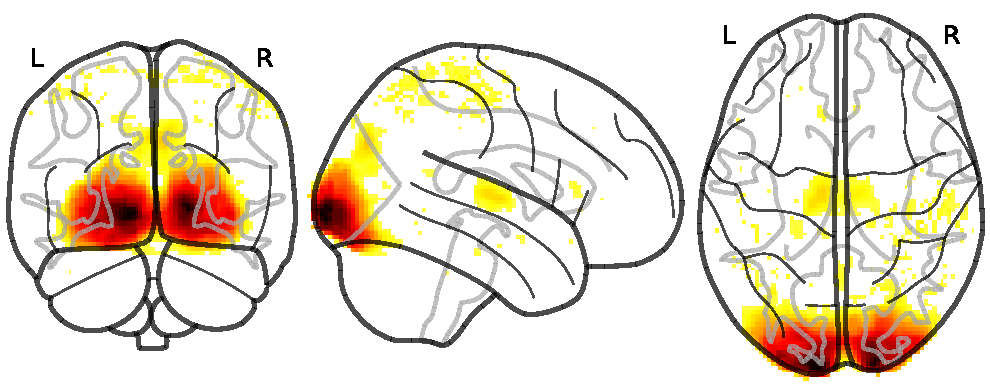
\includegraphics[width=0.38\textwidth]{fig/hcp/RSN_components/RSN_01}}
  \subcaptionbox{3: Visual (Lateral, Cognition–Space) \label{fig:rsn-3}}{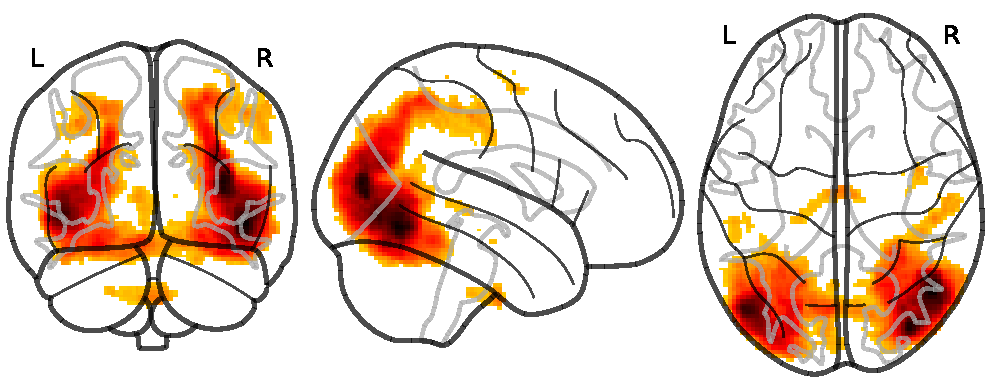
\includegraphics[width=0.38\textwidth]{fig/hcp/RSN_components/RSN_02}}
  \hspace{0.08\textwidth}
  \subcaptionbox{4: Default Mode Network (DMN) \label{fig:rsn-4}}{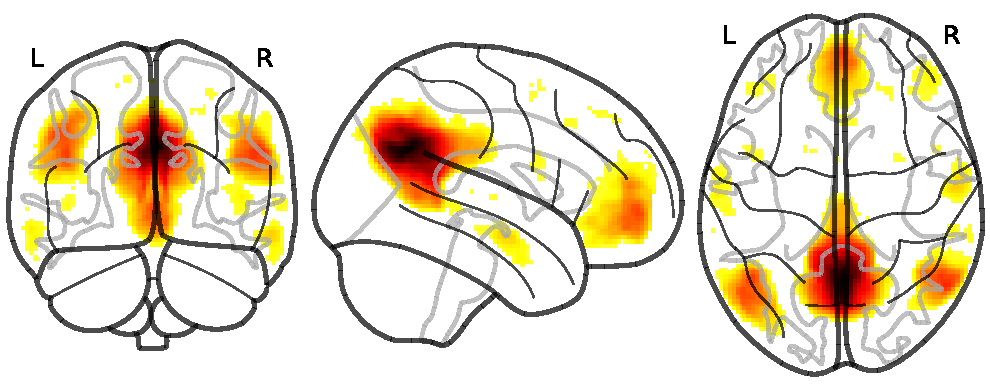
\includegraphics[width=0.38\textwidth]{fig/hcp/RSN_components/RSN_03}}
  \subcaptionbox{5: Cerebellum (CBM) \label{fig:rsn-5}}{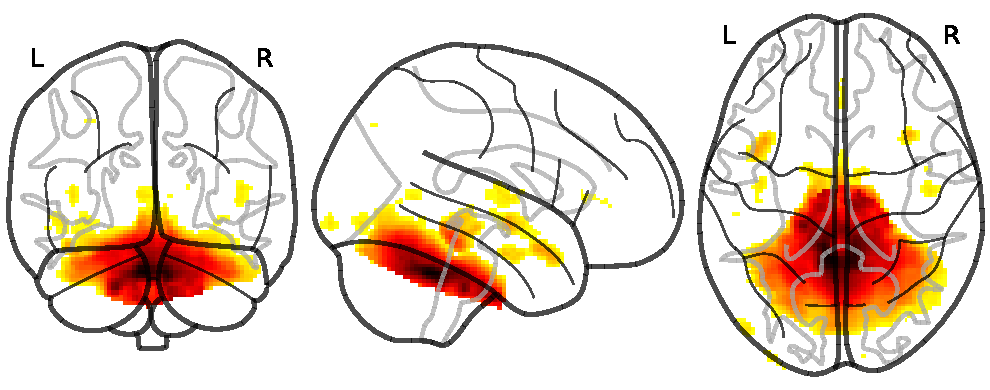
\includegraphics[width=0.38\textwidth]{fig/hcp/RSN_components/RSN_04}}
  \hspace{0.08\textwidth}
  \subcaptionbox{6: Sensorimotor (SM) \label{fig:rsn-6}}{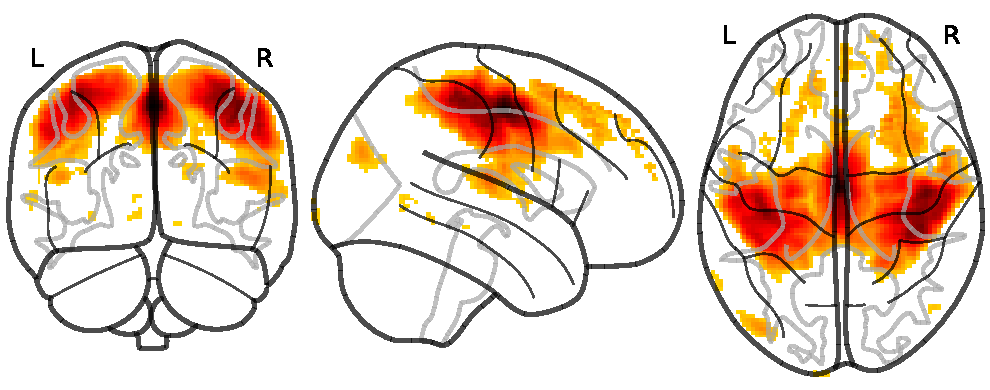
\includegraphics[width=0.38\textwidth]{fig/hcp/RSN_components/RSN_05}}
  \subcaptionbox{7: Auditory (AUD) \label{fig:rsn-7}}{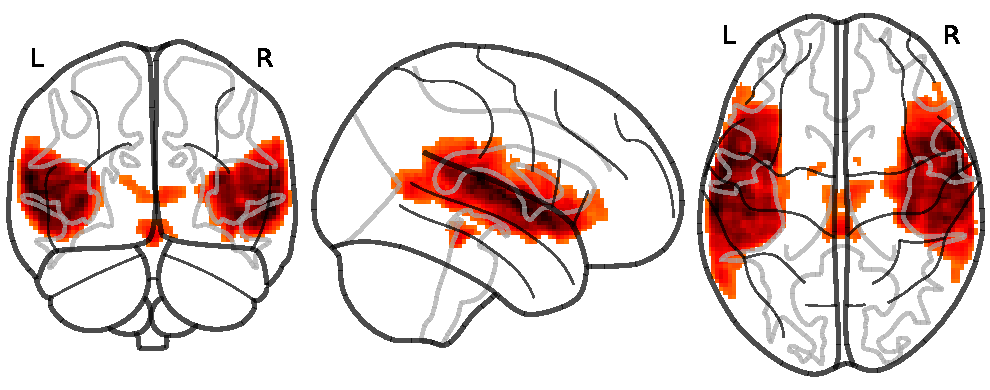
\includegraphics[width=0.38\textwidth]{fig/hcp/RSN_components/RSN_06}}
  \hspace{0.08\textwidth}
  \subcaptionbox{8: Executive Control (EC) \label{fig:rsn-8}}{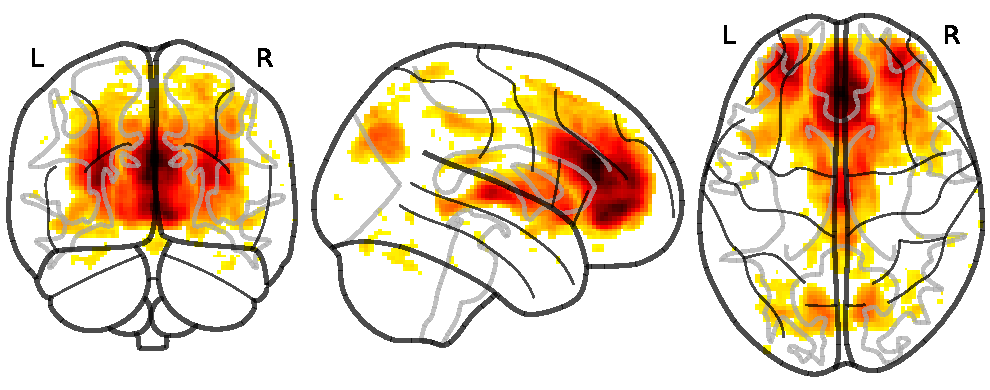
\includegraphics[width=0.38\textwidth]{fig/hcp/RSN_components/RSN_07}}
  \subcaptionbox{9: Frontoparietal (Perception-Somesthesis-Pain) \label{fig:rsn-9}}{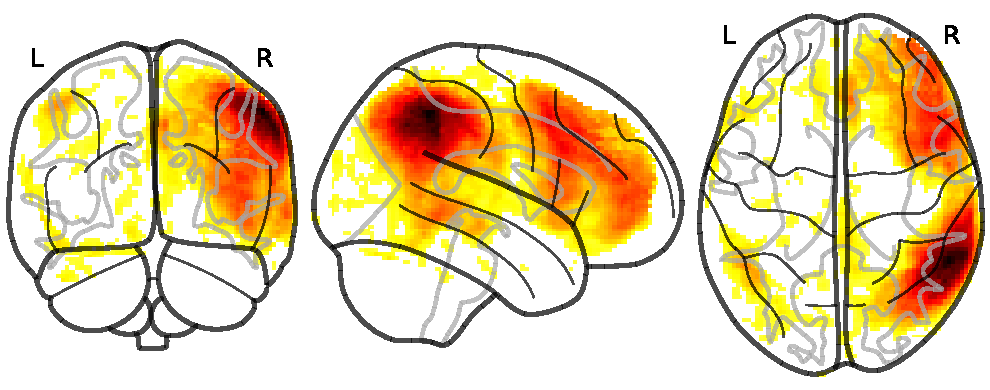
\includegraphics[width=0.38\textwidth]{fig/hcp/RSN_components/RSN_08}}
  \hspace{0.08\textwidth}
  \subcaptionbox{10: Frontoparietal (Cognition-Language) \label{fig:rsn-10}}{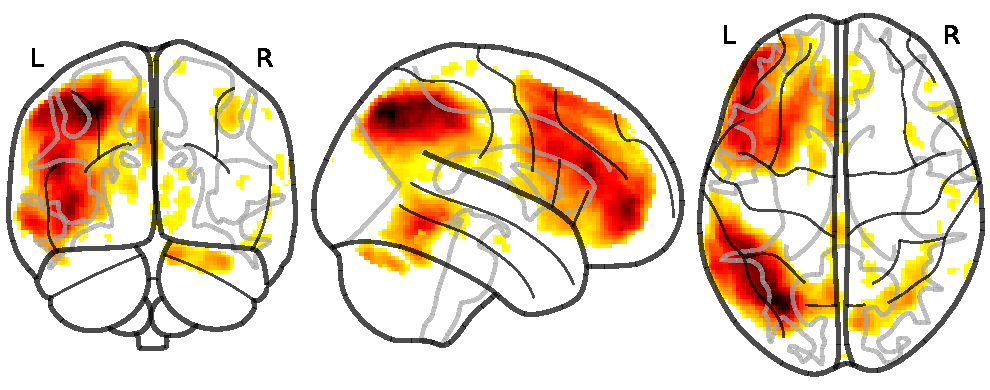
\includegraphics[width=0.38\textwidth]{fig/hcp/RSN_components/RSN_09}}
  \caption{
    Functional networks from \textcite{Smith2009}.
  }
  \label{fig:brainmap-functional-networks}
\end{figure}

% Add back a), b), etc.
\captionsetup[subfigure]{labelformat=simple, labelsep=colon}  % or parens?


Each subject undergoes four scans in total, divided into two consecutive scans on two separate days.
We will refer to these scans as 1A, 1B, 2A, and 2B.
We only include subjects for which all of these four scans are available, resulting in 812 subjects in total.
Scans were acquired with a \gls{tr} of 0.72 seconds and voxel size of 2~mm isotropic.
Each scan contains $N = 1200$ images and is 15 minutes long.
%
Data was preprocessed by the \gls{hcp} team according to the (minimal) preprocessing pipeline using \gls{fsl}~\parencite{Jenkinson2012} and FreeSurfer~\parencite{Fischl2012}.
The pipeline is described in more detail in \textcite{Jenkinson2002, Glasser2013, Smith2013a, Smith2013b}.
Importantly, noise components have been filtered out during preprocessing using ICA+FIX~\parencite{Salimi2014, Griffanti2014}.
This ensured that none of the components we use can be considered as a noise component.
All time series were also demeaned and variance normalized~\parencite{Beckmann2004}.
All \gls{ica} components for each subject and for each scan were individually standardized to have zero mean and unit variance.
For more data preprocessing details we refer the reader to the \gls{hcp} release manual.

%%
\subsubsection{Subject measure prediction benchmark}
%%

One common benchmarking approach is to investigate the predictive power of subject measures (i.e.~phenotypes, such as subject age) from \gls{tvfc} estimates from the different methods, using regressors and classifiers.
This makes sense on multiple levels.
We know that individual differences are contained in \gls{rs-fmri} scans~\parencite{Finn2015}.
Furthermore, subject measure prediction is similar to many practical use cases of \gls{tvfc} estimates, for example when used in clinical contexts for disease diagnosis and prognosis.
%
The idea here is as follows.
If a method's estimated covariance structure has more predictive power than another's, it can be said it has extracted and preserved more relevant information (for that particular prediction task at hand).
It is likely that some methods preserve more relevant information for some tasks, yet other methods preserve more for other tasks.
However, we can look at the average across many subject measures, or we may suggest which method to use after selecting a subject measure of interest.
As such this benchmarking can be considered a `profiling' or `cataloging' exercise.
Here we investigate the task of predicting subject measures for subjects from the \gls{hcp} data set.

\info[inline]{Paragraph: Describe morphometricity algorithm.}
Estimated covariance structure and subject measures are related through a \textbf{morphometricity} analysis~\parencite{Sabuncu2016}, using the variance component model.
This model, based on \gls{lme} modeling, finds a linear relationship between estimated \gls{tvfc} and subject measures.
\textcite{Sabuncu2016} defined this global metric of morphometricity as the proportion of phenotypic variation that can be explained by macroscopic brain morphology (i.e.~inter-subject anatomical variation).
The score has a value between 0 and 1, with 1 explaining all variance.
Their original study looked at anatomical variation between subjects.
Therefore, in their context this score is a measure of the anatomical signature of a certain trait.

Scores are computed as follows.
We posit for following model:
\begin{equation}
  \mathbf{y} = \mathbf{X} \mathbf{\beta} + \mathbf{a} + \mathbf{\epsilon},
  \label{eq:lme}
\end{equation}
where $\mathbf{y}$ is a column vector of length equal to the number of subjects studied containing, some quantitative subject measure (e.g.~age), $\mathbf{X}$ is the design matrix of confounding variables (a.k.a.~covariates or nuisance variables) weighted by~$\mathbf{\beta}$, $\mathbf{a}\sim \mathcal{N}(\mathbf{0}, \sigma_a^2 \mathbf{K}_a)$ is a random effects vector, and $\mathbf{\epsilon} \sim \mathcal{N}(\mathbf{0}, \sigma_e^2)$ is a noise vector.
We call the symmetric matrix $\mathbf{K}_a$ the \gls{tvfc} similarity matrix (in contrast with the original paper, where it is called the \emph{anatomical} similarity matrix).
Each value in this matrix encodes how globally `similar' two particular subjects are.
It is still our choice how to define similarity in this case based on \gls{tvfc} estimates.
More specifically then, morphometricity is computed as
\begin{equation}
  m^2 = \frac{\sigma_a^2}{\sigma_a^2 + \sigma_e^2} = \frac{\sigma_a^2}{\sigma_y^2},
\end{equation}
where $\sigma_y^2$ is called the phenotypic variance.
In order words, morphometricity is the amount of phenotypic variation that can be explained by variation in \gls{tvfc} estimates.
Parameters~$\sigma_a^2$ and~$\sigma_e^2$ are estimated using the \gls{reml} method~\parencite{Patterson1971, Harville1977}.
We can use this in our model comparison framework as follows: methods whose \gls{tvfc} estimates can explain more subject phenotypic variation can be considered superior.

\info[inline]{Paragraph: Define subject-by-subject similarity matrix.}
How should we define the similarity $\mathbf{K}_a$ between subjects?
In our analysis we re-purpose the morphometricity analysis and consider subject `similarity' as indicated by whole-brain estimated \gls{tvfc}.
Instead of using the full $N \times D \times D$ estimated covariance structure, we use the $D \times D$ dimensional summary measures of it.
The summary measures are the mean, variance, and rate-of-change of \gls{tvfc} estimates, as discussed in \cref{subsec:tvfc-summary-measures}.
This can be viewed as a feature or biomarker extraction step.
We take the lower triangular values as a vector of size $\frac{D(D-1)}{2}$, excluding the diagonal (self-connections) and duplicate values (since the matrices are symmetric).
Following \textcite{Sabuncu2016}, distance between subjects is defined by a Gaussian kernel, that is $k(\textbf{x}, \textbf{x}') = \exp(-(x-x')^2)$.

\info[inline]{Paragraph: Describe our subject measures.}
The variance component model relates \gls{tvfc} estimates to just a single phenotype or subject measure.
We repeat the analysis for a range of subject measures.
%
In fact, another study has run a similar analysis to benchmark \gls{fmri} data preprocessing.
In this work, \textcite{Li2019a} studied the predictive power of \gls{sfc} estimates after both including or excluding a crucial preprocessing pipeline researcher choice: whether to include \gls{gsr} or not.\footnote{The respective authors also implemented a regression on top of this, and find that the predictive power and the amount of variance explained are highly correlated concepts.}
They conclude that \gls{gsr} significantly increases the predictive power of \gls{sfc} estimates.
To allow for comparison and because they capture a wide range of individual differences, we study the exact same behavioral subject measures as they did: age, gender, and a range of cognitive task scores.
These subjects measures were investigated in a related study as well~\parencite{Kong2019}, where it was found that not only \gls{sfc} but also network topography has predictive power of such measures.
%
Age and gender are included as nuisance variables in our model, that is $\mathbf{X}$ in \cref{eq:lme}.
Some subject measures were missing from the raw data.
We filled missing values with mean imputation.
%
Furthermore, the same analysis is run on social-emotional and a range of other subject measures (including personality).
However, these are considered as less relevant, and their results have been moved to \cref{appendix:hcp-more-results}.

%%
\subsubsection{Test-retest robustness benchmark}
%%

Apart from a performance metric that captures how well methods can estimate covariance structures, we can also compare method \emph{robustness} across scans from the same subject.
Such robustness is another desired property of any \gls{tvfc} estimation method.
The idea here is that a method that predicts consistent subject attributes across scans should be more robust and would have captured some aspect of individual differences.

Here we broadly follow \textcite{Choe2017} and their test-retest study for \gls{tvfc} estimates in \gls{rs-fmri} data.
They studied the same data set, albeit an older and smaller version thereof.
%
Their idea was to test reliability of \gls{tvfc} summary measures derived from \gls{tvfc} methods.
In their study they looked at \gls{sw}, tapered \gls{sw}, and \gls{dcc} (i.e.~\gls{mgarch}) methods.
They evaluated these methods on two publicly available \gls{rs-fmri} data sets suitable for test-retest studies: the Multimodal MRI Reproducibility Resource (Kirby Data) and the \gls{hcp} Data.
The results for both data sets were found to be very consistent.
Therefore, we judged it sufficient to only consider data from the \gls{hcp}.
Their main finding was that the \gls{dcc} more reliably predicts \gls{tvfc} variance across sessions compared to the \gls{sw} methods.

Our study differs in a number of ways.
We only replicate these experiments for an updated and larger version of the \gls{hcp} data.
We include our additional models (i.e.~the \gls{svwp} and \gls{sw-cv}) as well as the additional rate-of-change \gls{tvfc} summary measure.
Moreover, we study the $D = 15$ case instead of their $D = 50$ case.
Interestingly, they ran the \gls{dcc} model by looping over all bivariate cases in the 50-dimensional \gls{ica} time series data (see also \cref{subsec:higher-dimensions}).
Therefore, we run both the joint and pairwise implementation of \gls{dcc}.

To quantity test-retest reliability, \glspl{icc} are computed for the estimated \gls{tvfc} summary measures separately for each individual edge~\parencite{Shrout1979, Chen2018}.
This \gls{icc} is computed as
\begin{equation}
  ICC = \frac{\sigma_X^2}{\sigma_X^2 + \sigma_U^2},
  \label{eq:icc}
\end{equation}
where $\sigma_X^2$ is the between-subject variance, and $\sigma_U^2$ is the within-subject variance.
%
In fact, several versions of \gls{icc} computation exist, and some controversies persist.
For example, \textcite{Noble2019} argued that \gls{icc}(3,1) should not be used in general, while \textcite{Chen2018} argued it can be.
We have opted to implement the most commonly used method in neuroimaging: \gls{icc}(2,1).
Scores are computed using the open-source Python package \texttt{pingouin}~\parencite[][version 0.5.2]{Vallat2018}.
Empirically we did not find large differences between \gls{icc}(1,1), \gls{icc}(2,1), and \gls{icc}(3,1) scores.

Furthermore, again following \textcite{Choe2017}, we compute I2C2 scores, which can be seen as a single omnibus representation for the whole brain~\parencite{Shou2013}.
This I2C2 score is computed as
\begin{equation}
  I2C2 = \frac{tr(\mathbf{K}_X)}{tr(\mathbf{K}_X + \mathbf{K}_U)},
  \label{eq:i2c2}
\end{equation}
where $\mathbf{K}_X$ is the between-subject covariance and $\mathbf{K}_U$ is the covariance of the replication error.

\textcite{Choe2017} also performed a similar test-retest study for brain states, extracting $k = 3$ brain states from the \gls{hcp} data using $k$-means clustering.
Interestingly, retest reliability here was poor for the \gls{dcc} method.

%%
\subsubsection{Brain states analysis}
%%

Brain states are extracted from the estimated \gls{tvfc} as described in \cref{sec:tvfc-feature-extraction}.
We extract $k = 3$ brain states, following \textcite{Choe2017} to allow for comparison.
However, there are better methods for determining the optimal number of clusters, either through non-parametric approaches~\parencite[see e.g.][]{Nielsen2017, Taghia2017} or by looking at a so-called `elbow plot'.
The latter plots the inertia (summed distance of each data point to its assigned cluster centroid) of each number of clusters proposed in $k$-means clustering.
The optimal number of clusters then is the one after which the inertia decreases linearly (i.e.~the number of clusters at the `elbow' of the line plot).

As described in \cref{subsec:brain-states}, brain state extraction is based on the hypothesis that functional organization is characterized by a sequence of discrete and distinct brain `connectivity' states.
When such states have been established across a population, it is common to compute dwell times or occupancy of states, defined as the fraction of time a given subject spent in each state.
We also compute the number of brain state change points (i.e.~switches).
This metric serves as an indication of how stable the state structure is for a given subject.

We do not consider the brain state analysis to be a proper benchmark for method selection, as it is not clear how to determine the superior \gls{tvfc} estimation method from this analysis.
Yet, it will be of interest to understand which estimation methods yield similar brain states, and what the main differences between methods are.
As such it helps us profile the \gls{tvfc} estimation methods discussed.

%%
\subsubsection{Implementational details}
%%

In terms of \gls{wp} models, we only run the \gls{svwp} model here with $M = 200$ inducing points, due to the large number of volumes per scan ($N = 1200$).

%%
\subsection{Task-based fMRI}
\label{subsec:rockland-methodology}
%%

\info[inline]{Paragraph: Introduce our tb-fMRI-based benchmark.}
Here we study how a visual \gls{tb-fmri} experiment can be used to benchmark \gls{tvfc} estimation methods.
We look at a single visual task experiment from the Rockland data set~\parencite{Nooner2012}.
%
It is worth remembering that \gls{tb-fmri} was the dominant paradigm in \gls{fmri} studies before the advent of \gls{rs-fmri}.
Intuitively it makes sense to use external stimuli to induce a desired response in the brain, as it grants researchers greater control and flexibility than in \gls{rs-fmri} settings.
However, even with a simple stimulus, the expected brain response is still often unclear.
Therefore, we only look at the most straightforward external stimulus experimental paradigm available.

How do we formulate a benchmark using this \gls{tb-fmri} data set?
Like the data in the \gls{rs-fmri} benchmarks, we do not have access to a ground truth covariance structure.
However, we do know all the specifics of the external signal from the task, which (again) can serve as a \emph{proxy} for ground truth.
That is, we evaluate methods in terms of how \emph{predictive} the \gls{tvfc} estimates are of the externally presented stimulus.
Crucially, this means we consider the node time series \emph{as is}.
We treat them as if we are unaware of the task paradigm.

%%
\subsubsection{Data: Rockland visual task}
\label{subsec:rockland-data}
%%

\info[inline]{Paragraph: Describe Rockland data.}
The Rockland data set consists of 286 subjects alternatingly either fixating in the dark or seeing a checkerboard visual pattern consecutively (20 seconds in duration of both stimuli and rest periods).
We only consider subjects between the ages of 18 and 35.
The checkerboard (moving) pattern is designed to continuously stimulate the visual cortex, while avoiding any adaptation effects (i.e.~reduced response after prolonged stimulation).
As further motivation for using this design, \textcite{Di2015} has shown that \gls{fc} is not static across such visual stimuli, and that \gls{fc} between higher and lower visual regions is affected in a consistent manner with stimulus on- and offset.
%
Two data sets are available, one collected with a \gls{tr} of 1.4~seconds ($N = 98$) and one with a \gls{tr} of 0.645~seconds ($N = 240$).
We only use the latter in these experiments.
Moreover, we only use data from the first baseline visit (coded \texttt{ses-BAS1}).

\info[inline]{Paragraph: Describe Rockland data preprocessing.}
Data preprocessing is run in \gls{fsl}~\parencite{Jenkinson2012}.
After brain extraction and field-of-view fixation, data was registered, motion corrected (i.e.~inter-slice corrected), smoothed with a Gaussian kernel with a \gls{fwhm} of 5~mm, and then detrended using a high-pass filter at 0.01~Hz.
No initial volumes are left out of the scan.
Finally, we de-noised the data using ICA-AROMA~\parencite{Pruim2015a, Pruim2015b}.
This is a method for Automatic Removal Of Motion Artifacts based on \gls{ica}.
It removes components deemed to be related to head motion from the data through linear regression.
Importantly, the data is not pre-whitened.
%
We know that \gls{v1} activation should correlate strongly with the external stimulus~\parencite{Sahib2018}.
Therefore, we discard subjects with a correlation between their \gls{v1} \gls{bold} time series and the stimulus (convolved with an \gls{hrf}) time series of below 0.4.
Such low correlation indicates the expected \gls{bold} signature in \gls{v1} was not observed (e.g.~possibly due to subjects closing their eyes, movement, or any other factor).

We extract \gls{bold} activations from visual areas \gls{v1}, V2, V3, V4, the \gls{mpfc}, and the \gls{m1} (Brodmann area 4; as control).
%
Individual node time series are noisy.
However, since we have an external cue that drives \gls{bold} signal measurements, we can (unlike with \gls{rs-fmri}) align all time series across subjects.
These average node time series are shown in \cref{fig:rockland-time-series-mean-over-subjects}.
Generally the \gls{bold} measurements in the visual regions track the external task well.
As expected, correspondence to the external stimulus decreases as we move up and away from the visual processing hierarchy.
In \gls{mpfc} and \gls{m1} regions, we see slight bumps in activity with stimulus on- and offset.


\begin{figure}[t]
  \centering
  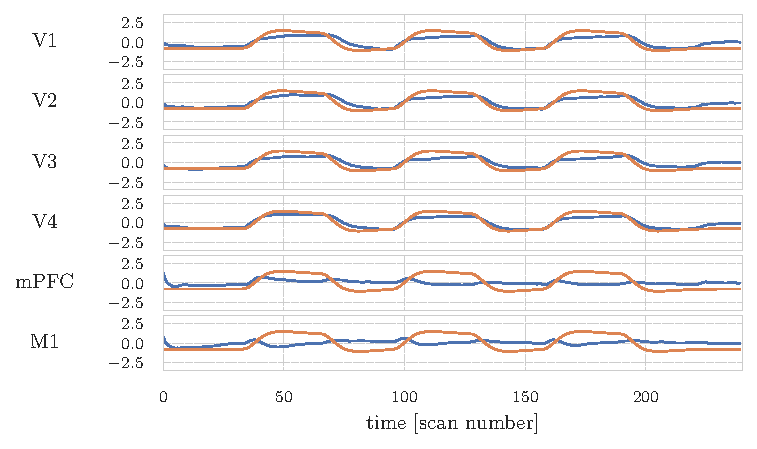
\includegraphics[width=\textwidth]{fig/rockland/CHECKERBOARD645/node_timeseries/mean_over_subjects}
  \caption{
    Rockland data normalized BOLD time series averaged over all 286 subjects.
    External visual stimulus convolved with HRF is shown for reference.
  }
  \label{fig:rockland-time-series-mean-over-subjects}
\end{figure}


Initially, we aim to extract a well-understood phenomenon, related to the hierarchy in the visual cortex.
Based on the hierarchical nature of the visual cortex, we expect \gls{v1} to correlate most strongly with V2, followed by V3 and V4.
But what about \gls{mpfc} and \gls{m1}?
In fact, we quickly run into a recurring issue in the field: circular analysis~\parencite{Kerr1998, Kriegeskorte2009, Kriegeskorte2010, Poldrack2012, Poldrack2017}.
This motivates other ways of defining this benchmark.

%%
\subsubsection{External stimulus prediction}
%%


\begin{figure}[t]
  \centering
  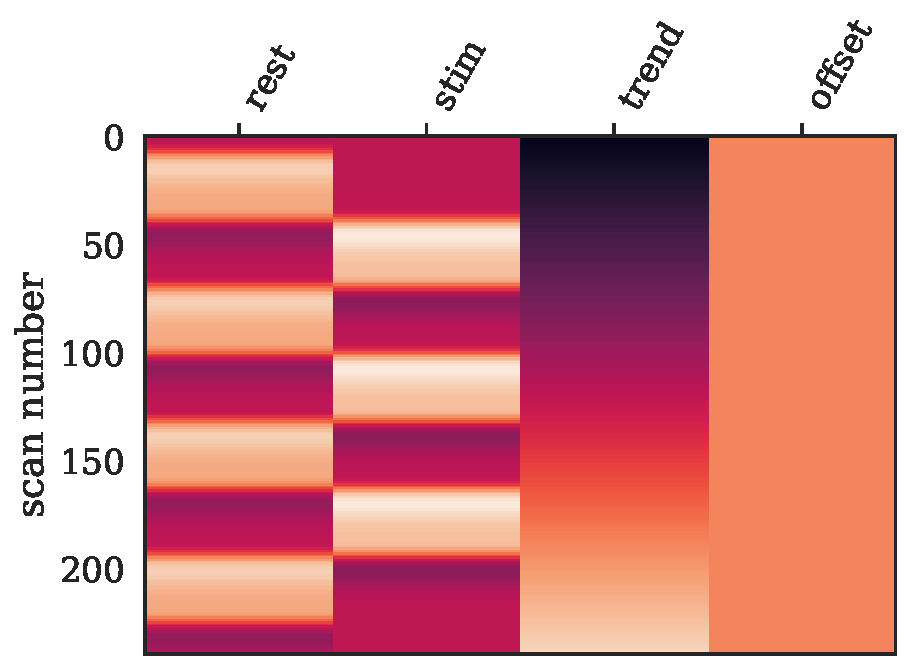
\includegraphics[width=0.6\textwidth]{fig/rockland/CHECKERBOARD645/prediction_benchmark/design_matrix_nilearn}
  \caption{
    Rockland benchmark design matrix $\mathbf{X}$ used for predicting external stimulus.
  }
  \label{fig:rockland-design-matrix}
\end{figure}


We frame our prediction task as predicting the presence of the external visual stimulus.
As we are in the domain of \gls{tb-fmri}, we can use a well-established technique based on the \gls{glm} and its \textbf{design matrix}.
The \gls{glm} is defined as
\begin{equation}
  \mathbf{Y} = \mathbf{X} \mathbf{\beta} + \mathbf{E},
\end{equation}
where $\mathbf{Y} \in \mathbb{R}^{G \times N}$ is the estimated \gls{tvfc} for a given method for all $G = 5$ edges of interest (i.e.~\gls{v1} connectivity with the other five \glspl{roi}),\footnote{This replaces the voxels by $N$ matrix used in typical \gls{fmri} studies~\parencite{Friston1995}.} $\mathbf{X} \in \mathbb{R}^{R \times N}$ is the design matrix with $R$ regressors (shown in \cref{fig:rockland-design-matrix}) weighted by $\beta \in \mathbb{R}^{R \times G}$, and $\mathbf{E} \in \mathbb{R}^{G \times N}$ are the error terms.
%
The regressors in $\mathbf{X}$ are hypothesized contributors to the experiment.
They can be divided into `experimental' regressors (those of interest) and `nuisance' regressors (those we expect to affect the measurements but are not of interest, such as motion parameters or physiological signals as heart rate).
Our experimental regressors are the box-car (block design) model of the visual stimulus, convolved with the \gls{hrf}~\parencite{Glover1999}.
Our nuisance regressors are first-order polynomials.
The polynomial (drift) order was determined as \gls{tr} multiplied by~$\frac{N}{150}$~\parencite[see][for rationale]{Worsley2002}.
Effectively this reduces to allowing the model to \emph{detrend} the observed \gls{tvfc} estimates (this includes a constant value as well to remove the \emph{offset}).
Adding these can be considered similar to actively detrending the \gls{tvfc} estimates (e.g.~using bandpass filtering), but adding them to the design matrix allows the model to learn the relevance automatically.
This matrix is generated and plotted using the open-source Python library \texttt{Nilearn}~\parencite[][version~0.9.2]{Abraham2014}, which in turn is built upon \texttt{scikit-learn}~\parencite[][version~1.1.1]{Pedregosa2011} and \texttt{SciPy}~\parencite[][version~1.8.0]{SciPy2020}.
We infer $\mathbf{\beta}$ from the observations using \gls{ols} to minimize the error terms~$\mathbf{E}$~\parencite{Worsley1995}.
These $\beta$ parameters can then be used to determine which \gls{tvfc} estimates have captured the presence of the external visual stimulus best.
Entries in this regressor matrix indicate relative contributions of regressors in predicting $\mathbf{Y}$.

%%
\subsubsection{Implementational details}
%%

We only train the \gls{vwp} here, as $N$ is reasonably small.
